\documentclass[10pt,twocolumn]{article}
\usepackage[letterpaper,margin=0.7in,columnsep=0.25in]{geometry}
\usepackage[T1]{fontenc}
\usepackage{lmodern}
\usepackage{microtype}
\usepackage{graphicx}
\usepackage{booktabs}
\usepackage{amsmath}
\usepackage[font=small,labelfont=bf,skip=4pt]{caption}
\usepackage{subcaption}
\usepackage[hidelinks]{hyperref}
\graphicspath{{../results/figures/}}
\setlength{\textfloatsep}{8pt plus 2pt minus 2pt}
\setlength{\dbltextfloatsep}{8pt plus 2pt minus 2pt}
\setlength{\tabcolsep}{4pt}

% Every number in this report comes from results/tables/*.md (see results/tables/headline.md).

\title{\vspace{-0.6in}\Large LabelLite: Label-Efficient, Uncertainty-Aware Image Classification\\
with Frozen Foundation Models}
\author{}
\date{}

\begin{document}
\maketitle
\vspace{-0.55in}

\begin{abstract}
\noindent
Expert labels are expensive in pathology and remote sensing, and a model used there has to be
able to flag the predictions it cannot back up. We benchmark four frozen vision backbones (ResNet-50, DINOv2, CLIP, and
the pathology model Phikon) with linear probes against a fully fine-tuned ResNet-50 on
PatchCamelyon (PCam) and EuroSAT at 1\%, 10\% and 100\% of training labels, and add temperature
scaling, split-conformal triage, a synthetic stain shift, and simulated active learning. On
PCam, a linear probe on Phikon features trained on 1\% of the labels (AUROC 0.980) outperforms
the ResNet-50 fine-tuned on all labels (0.966). Conformal triage auto-labels 90.1\% of PCam test
patches at a 95\% coverage target with 4.7\% error among them, but coverage falls short by up to
4.7 points because calibration and test slides differ, and further under stain shift. On
EuroSAT, uncertainty sampling reaches random sampling's final accuracy with 58--65\% fewer
labels; on PCam it does not help. This is a research benchmark and makes no clinical claims.
\end{abstract}

\section{Introduction}
Labeled data in pathology and remote sensing is expensive because it needs a domain expert.
Self-supervised foundation models promise useful features without task labels, and conformal
prediction promises a distribution-free way to decide which predictions to trust. We ask five
questions on two image domains: whether frozen features plus a linear probe match a fine-tuned
CNN at low label budgets (RQ1); whether their confidences are calibrated (RQ2); whether
split-conformal triage can auto-label images at a controlled error (RQ3); how these properties
hold under a stain shift (RQ4); and whether uncertainty-driven active learning saves labels
(RQ5). All code, configurations, split IDs and result tables are released; every number below
is produced by the pipeline.

\section{Related work}
\paragraph{Frozen features and foundation models.} Linear probes on frozen features are a
standard test of representation quality, and ImageNet accuracy predicts transfer only
partly~\cite{kornblith2019}. Self-supervised models such as DINOv2~\cite{oquab2023} and
language-supervised CLIP~\cite{radford2021} are evaluated this way on natural images. In
pathology, self-supervised models trained on large slide collections, among them
Phikon~\cite{filiot2023}, UNI~\cite{chen2024} and CONCH~\cite{lu2024}, report strong linear-probe
results on patch-level pathology benchmarks. We compare general-purpose and pathology models
\emph{across} domains, and against fine-tuning at matched label budgets.

\paragraph{Calibration and conformal prediction.} Modern networks are often overconfident, and
temperature scaling is a simple post-hoc fix~\cite{guo2017}. Split conformal
prediction~\cite{vovk2005,angelopoulos2021} turns any classifier into set-valued predictions with
marginal coverage under exchangeability. LAC~\cite{sadinle2019} gives the smallest sets on
average, while APS~\cite{romano2020} and RAPS~\cite{angelopoulos2021raps} aim for more adaptive
sets. Coverage guarantees break under distribution shift unless it is modeled, for example by
weighting for covariate shift~\cite{tibshirani2019}. Uncertainty estimates in general degrade
under shift~\cite{ovadia2019}. We measure this with fixed thresholds as a deployment would.

\paragraph{Shift in pathology.} Stain and scanner differences across hospitals are a major
source of shift in histopathology. Stain augmentation and normalization are common
mitigations~\cite{tellez2019}. Camelyon17~\cite{bandi2019} and its WILDS version~\cite{koh2021}
provide real cross-hospital splits. We use a controlled stain perturbation~\cite{ruifrok2001}
instead (Section~\ref{sec:limits}).

\paragraph{Active learning.} Uncertainty sampling~\cite{settles2009}, Bayesian
acquisition~\cite{gal2017} and diversity-based core-set selection~\cite{sener2018} are the main
families. We test the simplest uncertainty and core-set strategies, plus conformal set size, on
top of frozen features, where retraining a probe each round is cheap.

\section{Method}
\paragraph{Data.} PCam~\cite{veeling2018} has 327,680 H\&E lymph-node patches
($96\times96$\,px, binary tumor label) with official train/valid/test splits from disjoint
slides. EuroSAT RGB~\cite{helber2019} has 27,000 Sentinel-2 images ($64\times64$\,px, 10
land-cover classes) without official splits; we use a fixed stratified 60/10/10/20
train/val/cal/test split. The PCam calibration split is the official valid split (32,768); its
test split (32,768) comes from other slides. Label budgets of 1\% and 10\% are class-stratified
subsets of train, drawn with 3 seeds.

\paragraph{Models.} Frozen backbones: ResNet-50~\cite{he2016} (ImageNet-1k), DINOv2
ViT-B/14~\cite{oquab2023}, CLIP ViT-B/16~\cite{radford2021}, and Phikon~\cite{filiot2023}, an
iBOT ViT-B/16 pretrained on TCGA (an open substitute for gated pathology models; no Camelyon
slides in pretraining). Images are resized to $224\times224$ and features cached in float16. On
L2-normalized features we fit an L2-regularized logistic regression (C chosen on val) and a
$k$-NN classifier ($k=20$), and evaluate CLIP zero-shot. The baseline is ResNet-50 fully
fine-tuned with AdamW (warm-up, cosine decay), color jitter and early stopping on val, in bf16.

\paragraph{Calibration and conformal triage.} The calibration split is halved (stratified):
one half fits a temperature~\cite{guo2017}, the other calibrates split conformal
prediction~\cite{vovk2005,angelopoulos2021} on temperature-scaled probabilities with the LAC
score $1-\hat p_y$~\cite{sadinle2019} and randomized APS~\cite{romano2020}, at
$\alpha\in\{0.1,0.05\}$. An image whose set has exactly one class is auto-labeled; otherwise it
is routed to an expert. We report coverage, mean set size, the auto-labeled share, the error
among auto-labeled images, and system error (wrong auto-labels over all images, $\le\alpha$ if
the expert is always right). Coverage is compared with its exact finite-sample distribution
under exchangeability (calibration Beta law plus test binomial noise); as a control we also
calibrate on a random half of test.

\paragraph{Stain shift.} For RQ4, PCam test patches are shifted in Ruifrok--Johnston
optical-density stain space~\cite{ruifrok2001}: at severity $s\in\{1,2,3\}$ hematoxylin is scaled
by $1-0.15s$ and eosin by $1+0.25s$. These values were fixed by inspecting example images before
any shifted results existed. Models, temperatures and conformal thresholds stay fixed from
clean data.

\paragraph{Active learning.} Starting from the 1\% subset, 10 rounds each add 1\% of the train
pool, chosen by random sampling, least confidence, entropy, LAC conformal set size
($\alpha=0.1$, ties broken randomly), or $k$-center greedy~\cite{sener2018} on DINOv2 and Phikon
features. The oracle is the dataset label; 3 seeds per strategy.

\paragraph{Explanations.} Grad-CAM~\cite{selvaraju2017} of the predicted class's
log-probability, at ResNet-50's \texttt{layer4} and at the patch tokens entering each ViT's last
block, with the linear probe as a differentiable head. Maps are used qualitatively only.

\section{Results}

\begin{table}[t]
\centering\small
\caption{Test performance (mean $\pm$ std over 3 seeds at 1\%, 10\%; single run at 100\%).
PCam: AUROC. EuroSAT: accuracy. LP = linear probe, FT = fine-tuned.}
\label{tab:main}
\begin{tabular}{@{}lccc@{}}
\toprule
PCam AUROC & 1\% & 10\% & 100\% \\
\midrule
ResNet-50 LP & .907$\pm$.004 & .914$\pm$.002 & .913 \\
ResNet-50 FT & .922$\pm$.006 & .953$\pm$.004 & .966 \\
DINOv2 LP & .927$\pm$.003 & .936$\pm$.001 & .941 \\
CLIP LP & .900$\pm$.002 & .906$\pm$.001 & .910 \\
Phikon LP & \textbf{.980}$\pm$.001 & \textbf{.979}$\pm$.005 & \textbf{.982} \\
\midrule
EuroSAT accuracy & 1\% & 10\% & 100\% \\
\midrule
ResNet-50 LP & .870$\pm$.001 & .939$\pm$.002 & .966 \\
ResNet-50 FT & .865$\pm$.001 & \textbf{.968}$\pm$.002 & \textbf{.984} \\
DINOv2 LP & \textbf{.880}$\pm$.012 & .939$\pm$.002 & .965 \\
CLIP LP & .862$\pm$.007 & .930$\pm$.003 & .958 \\
Phikon LP & .792$\pm$.003 & .904$\pm$.004 & .952 \\
\bottomrule
\end{tabular}
\end{table}

\paragraph{RQ1: label efficiency.} Table~\ref{tab:main} and Fig.~\ref{fig:le}. On PCam, Phikon
dominates at every budget, and its 1\% probe (accuracy 0.925, AUROC 0.980) beats the ResNet-50
fine-tuned on 100\% of labels (0.886, 0.966). At 100\% labels the accuracy gap (+0.038) is
significant (McNemar, Holm-corrected $p<0.001$); the paired bootstrap of the AUROC gap
($+0.016$) gives $p=0.072$, the smallest value reachable with 1,000 resamples after Holm
correction over 36 pairs, so that test is underpowered rather than negative. On EuroSAT,
general-purpose features win at 1\% (DINOv2 0.880 vs.\ fine-tuned 0.865), fine-tuning wins from
10\% on, and the best probe at 10\% reaches 95.5\% of the fine-tuned model's full-label
accuracy (0.939 vs.\ 0.984). The pathology model is the weakest probe on satellite images, and
general-purpose models are far behind Phikon on pathology: domain-specific pretraining matters
in its own domain only. CLIP zero-shot is at chance on both datasets (accuracy 0.488 on PCam,
0.504 on EuroSAT) with our prompts.

\begin{figure*}[t]
\centering
\begin{subfigure}{0.40\linewidth}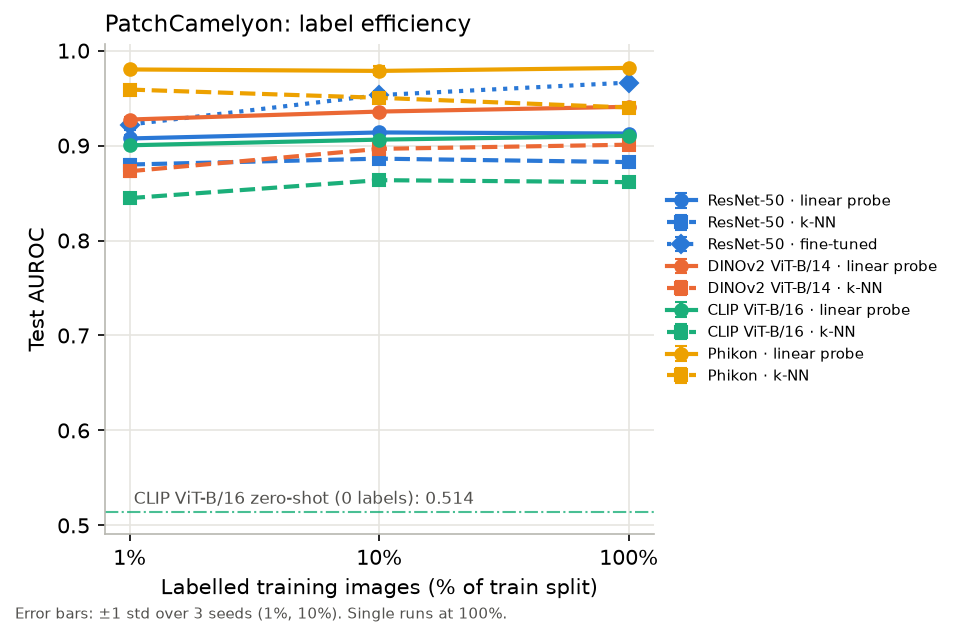
\includegraphics[width=\linewidth]{label_efficiency_pcam.png}\end{subfigure}\hspace{0.04\linewidth}%
\begin{subfigure}{0.40\linewidth}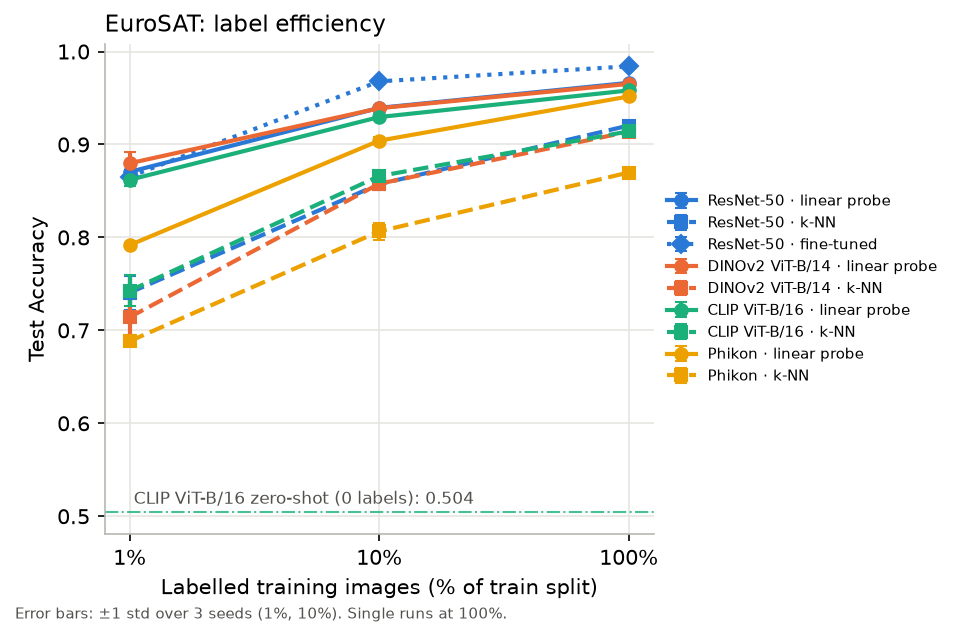
\includegraphics[width=\linewidth]{label_efficiency_eurosat.png}\end{subfigure}
\caption{Label efficiency: test AUROC on PCam (left) and accuracy on EuroSAT (right) against the
fraction of training labels, mean $\pm$ std over seeds.}
\label{fig:le}
\end{figure*}

\paragraph{RQ2: calibration.} Linear probes from 10\% labels up have expected calibration
error (ECE, 15 bins) of at most 0.035 before any correction. Miscalibration appears in the
low-label and fine-tuned regimes: the fine-tuned ResNet-50 on PCam has ECE $0.115\pm0.014$ at
1\% labels and 0.056 at 100\% (temperatures 2.58 and 2.00, i.e.\ overconfident), reduced by
temperature scaling to $0.028\pm0.005$ and 0.010. On EuroSAT at 1\% labels both ResNet-50
variants start near 0.15 and drop to 0.017--0.024. Phikon on PCam is already calibrated (ECE
0.007--0.013) and temperature scaling leaves it at 0.010--0.014.

\begin{table}[t]
\centering\small
\caption{Conformal triage at 10\% labels, LAC score (mean over 3 seeds, \%). Cov.\ = coverage;
Auto = auto-labeled share; Err = error among auto-labeled; Sys = system error.}
\label{tab:conf}
\begin{tabular}{@{}llcccc@{}}
\toprule
Target & Model & Cov. & Auto & Err & Sys \\
\midrule
\multicolumn{6}{@{}l}{\emph{PCam}} \\
95\% & Phikon LP & 95.8 & 90.1 & 4.7 & 4.2 \\
95\% & DINOv2 LP & 95.3 & 73.2 & 6.4 & 4.7 \\
95\% & ResNet-50 FT & 94.4 & 80.9 & 6.9 & 5.6 \\
90\% & Phikon LP & 90.4 & 96.8 & 6.6 & 6.4 \\
90\% & ResNet-50 FT & 88.1 & 98.3 & 12.1 & 11.9 \\
\midrule
\multicolumn{6}{@{}l}{\emph{EuroSAT}} \\
95\% & DINOv2 LP & 95.7 & 95.5 & 4.2 & 4.0 \\
95\% & ResNet-50 FT & 94.6 & 96.1 & 1.6 & 1.5 \\
90\% & DINOv2 LP & 90.5 & 93.9 & 3.6 & 3.4 \\
\bottomrule
\end{tabular}
\end{table}

\paragraph{RQ3: conformal triage.} Table~\ref{tab:conf}. With Phikon at a 95\% target, 90.1\%
of PCam test patches receive a single-label set, with 4.7\% error among them and 4.2\% system
error. APS produces larger sets: 73.3\% auto-labeled at 3.4\% error for the same model. On
EuroSAT, coverage lies within 3 standard deviations of its expected value in all 144 (run,
score, $\alpha$) cases. On PCam this holds in only 94 of 144, with deviations from $-4.7$ to
$+1.3$ points; calibrating on a random half of test instead restores 144 of 144. The gap is
therefore due to the slide-level difference between PCam's valid and test splits, a mild
shift that already violates exchangeability. Class-conditional coverage is uneven: at 10\%
labels and a 90\% target, the least-covered class sits as low as 73.9\% (Phikon LAC on EuroSAT)
and LAC under-covers tumors on PCam (e.g.\ 83.6\% for Phikon), whereas APS keeps the minimum
class coverage closer to target (87.7\% and 87.8\% for the same settings).

\begin{figure*}[t]
\centering
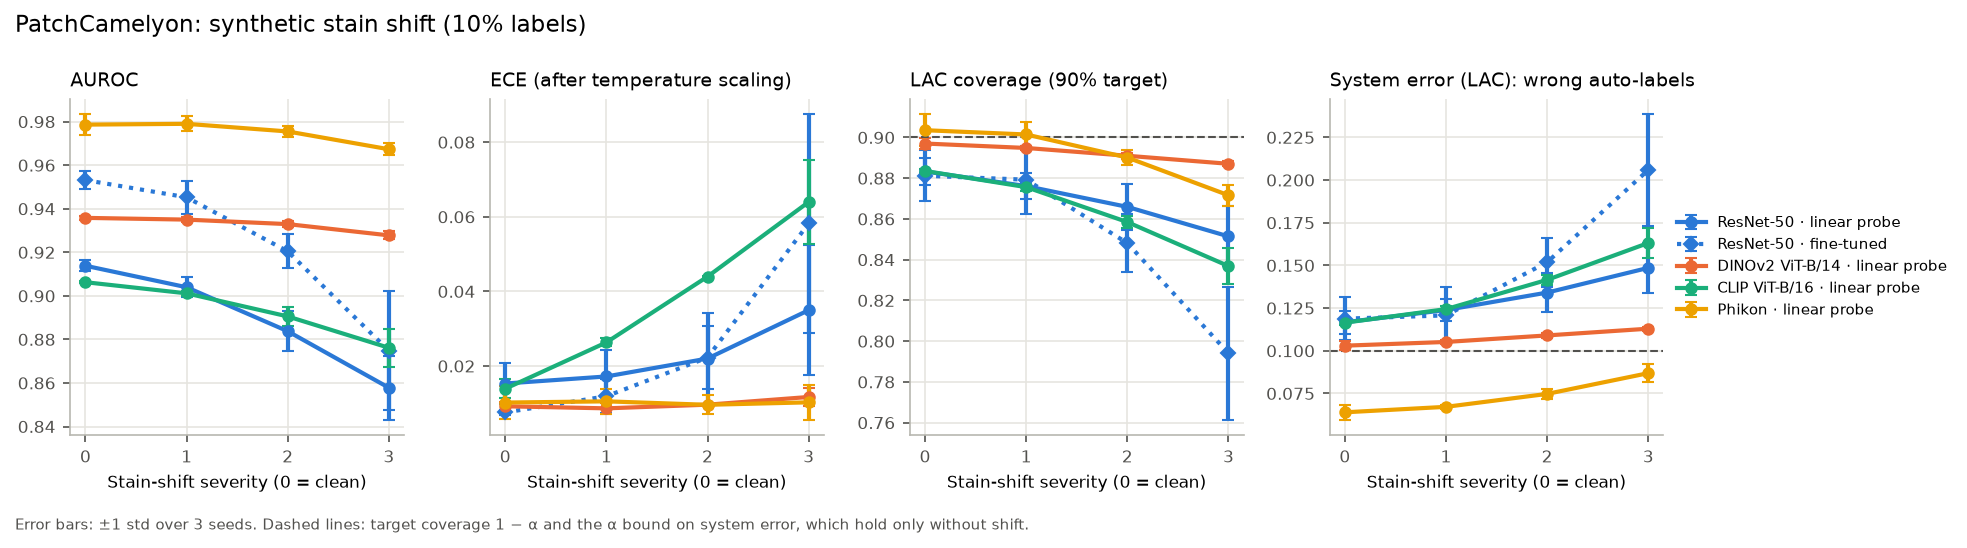
\includegraphics[width=0.92\linewidth]{shift_pcam.png}
\caption{Synthetic stain shift on PCam (10\% labels): metrics against severity, with models,
temperatures and conformal thresholds fixed from clean images.}
\label{fig:shift}
\end{figure*}

\paragraph{RQ4: stain shift.} Fig.~\ref{fig:shift}. From severity 0 to 3 (10\% labels, LAC at a
90\% target), the fine-tuned ResNet-50 degrades most: AUROC $0.953\to0.875$, coverage
$88.1\to79.4\%$, and system error $11.9\to20.6\%$. Frozen DINOv2 features are the most stable
(AUROC $0.936\to0.928$, coverage $89.7\to88.7\%$), Phikon remains the most accurate
($0.979\to0.967$; coverage $90.4\to87.2\%$), and CLIP and ResNet-50 probes lose 4.7 and 3.2
coverage points. APS degrades less than LAC for every frozen probe (e.g.\ DINOv2 stays at
90.0\%). Temperature-scaled ECE stays below 0.02 for DINOv2 and Phikon but reaches
$0.064\pm0.011$ for CLIP. Conformal thresholds set on clean data do not carry their guarantee
across a stain change, and the size of the failure depends strongly on the representation.

\begin{figure}[t]
\centering
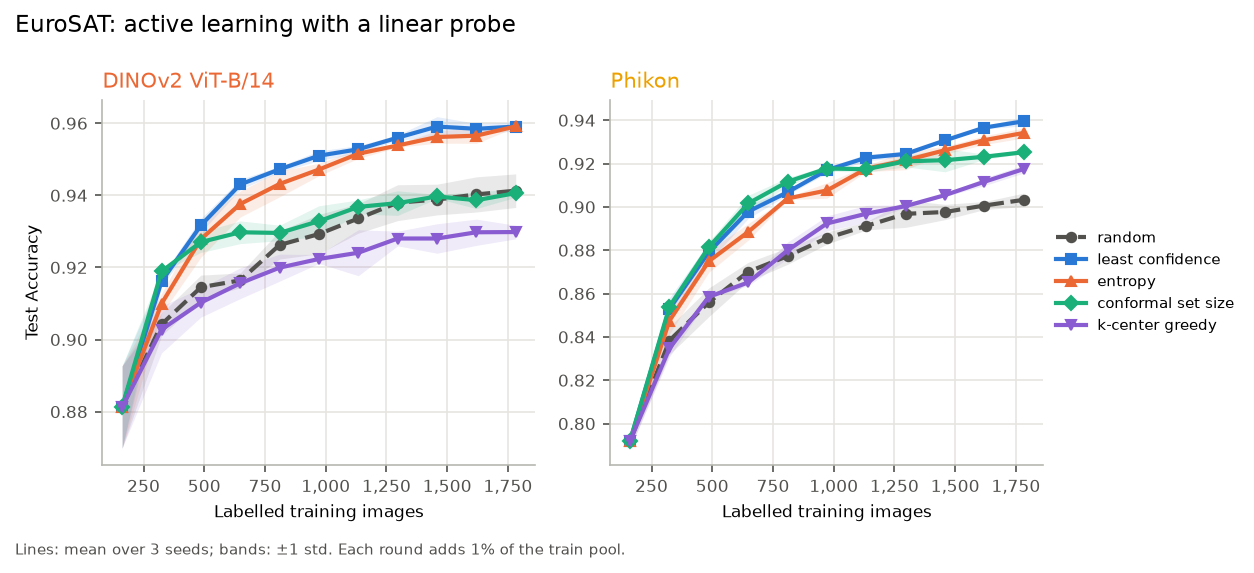
\includegraphics[width=\linewidth]{active_learning_eurosat.png}
\caption{Active learning on EuroSAT: test accuracy against labeled images (mean $\pm$ std over 3
seeds), DINOv2 (left) and Phikon (right).}
\label{fig:al}
\end{figure}

\paragraph{RQ5: active learning.} Fig.~\ref{fig:al}. On EuroSAT, least-confidence sampling ends
at 0.959 (DINOv2) and 0.940 (Phikon) accuracy against 0.941 and 0.903 for random sampling at
1,782 labels, and reaches random's final accuracy with 623 and 746 labels: 65\% and 58\% fewer
labels than random itself needs. Entropy is close behind (58\%, 55\%); conformal set size
saves 62\% with Phikon but never reaches random with DINOv2. On PCam no strategy beats random:
AUROC is flat from the 1\% start (Phikon random 0.982), and least confidence (0.975), entropy
(0.977) and $k$-center (0.965) end below it; a plausible but untested explanation is that
uncertainty sampling concentrates on ambiguous patches once the classifier has saturated. $k$-center greedy is the weakest
strategy in three of four settings.

\section{Failure modes}
The dominant PCam error of the reference Phikon probe (10\% labels, seed 0) is the costly one:
87.3\% of its 2,491 test errors are tumor patches predicted normal. On EuroSAT, the most
frequent DINOv2 confusions are between visually similar classes: AnnualCrop and PermanentCrop
(55 of 320 errors) and Highway and River (37).

In addition, 100 random errors per dataset were tagged by failure type, from each image and its
Grad-CAM map. No pathologist or remote-sensing expert was involved, so the counts describe what a
non-expert can see. On PCam, 57 of the 100 showed no tumor evidence a non-expert could
recognize; 17 were clear misses with visible clusters of larger cells; 10 had tissue only at the
patch edge; 7 had an adipose center, which points to coarse annotation; 7 were torn or blurred;
and 2 had unusual staining. EuroSAT errors are easier to read: 62 were look-alike classes,
mostly crop and vegetation types, 16 were mixed scenes containing both classes, 13 were plain
model errors, 5 had the defining feature in a small corner of the image, 2 looked mislabeled and
2 had haze or a color cast. The Grad-CAM galleries of confident errors and uncertain images are
released with the code. The ViT maps are limited to a $14\times14$ or $16\times16$ patch grid and
should not be read as evidence of what the model relies on.

\section{Limitations}\label{sec:limits}
PCam's patch-level labels simplify slide-level diagnosis, and EuroSAT images are upsampled from
$64\times64$\,px. The stain shift is synthetic; the planned cross-hospital test
(Camelyon17-WILDS) was not available for download. Conformal guarantees are marginal and assume
exchangeability, which PCam's own splits already violate. The fine-tuned baseline uses one
fixed recipe, and fine-tuning was not part of the active-learning study, whose oracle is the
dataset label. Three seeds per budget, and pairwise tests on seed 0 only, limit the statistical
resolution.

\section{Ethics}
This is a benchmark on public datasets, not a diagnostic tool, and the pathology results make
no clinical claim; a high patch-level AUROC does not establish clinical usefulness, and the
model's dominant error, missed tumor, is the clinically costly direction. Coverage is an
average over images, not a per-patient guarantee, and fails under shift. Phikon's weights are
licensed for non-commercial research; weights and raw images are not redistributed.

{\footnotesize
\begin{thebibliography}{99}\setlength{\itemsep}{0pt}
\bibitem{angelopoulos2021} A.~N. Angelopoulos and S.~Bates. A gentle introduction to conformal
prediction and distribution-free uncertainty quantification. arXiv:2107.07511, 2021.
\bibitem{angelopoulos2021raps} A.~N. Angelopoulos, S.~Bates, J.~Malik, and M.~I. Jordan.
Uncertainty sets for image classifiers using conformal prediction. ICLR, 2021.
\bibitem{bandi2019} P.~B\'andi et al. From detection of individual metastases to classification
of lymph node status at the patient level: the CAMELYON17 challenge. IEEE TMI, 2019.
\bibitem{chen2024} R.~J. Chen et al. Towards a general-purpose foundation model for computational
pathology. Nature Medicine, 2024.
\bibitem{filiot2023} A.~Filiot et al. Scaling self-supervised learning for histopathology with
masked image modeling. medRxiv, 2023.
\bibitem{gal2017} Y.~Gal, R.~Islam, and Z.~Ghahramani. Deep Bayesian active learning with image
data. ICML, 2017.
\bibitem{guo2017} C.~Guo, G.~Pleiss, Y.~Sun, and K.~Q. Weinberger. On calibration of modern
neural networks. ICML, 2017.
\bibitem{he2016} K.~He, X.~Zhang, S.~Ren, and J.~Sun. Deep residual learning for image
recognition. CVPR, 2016.
\bibitem{helber2019} P.~Helber, B.~Bischke, A.~Dengel, and D.~Borth. EuroSAT: A novel dataset
and deep learning benchmark for land use and land cover classification. IEEE JSTARS, 2019.
\bibitem{koh2021} P.~W. Koh et al. WILDS: A benchmark of in-the-wild distribution shifts. ICML,
2021.
\bibitem{kornblith2019} S.~Kornblith, J.~Shlens, and Q.~V. Le. Do better ImageNet models transfer
better? CVPR, 2019.
\bibitem{lu2024} M.~Y. Lu et al. A visual-language foundation model for computational pathology.
Nature Medicine, 2024.
\bibitem{oquab2023} M.~Oquab et al. DINOv2: Learning robust visual features without
supervision. TMLR, 2024.
\bibitem{ovadia2019} Y.~Ovadia et al. Can you trust your model's uncertainty? Evaluating
predictive uncertainty under dataset shift. NeurIPS, 2019.
\bibitem{radford2021} A.~Radford et al. Learning transferable visual models from natural
language supervision. ICML, 2021.
\bibitem{romano2020} Y.~Romano, M.~Sesia, and E.~J. Cand\`es. Classification with valid and
adaptive coverage. NeurIPS, 2020.
\bibitem{ruifrok2001} A.~C. Ruifrok and D.~A. Johnston. Quantification of histochemical staining
by color deconvolution. Analytical and Quantitative Cytology and Histology, 2001.
\bibitem{sadinle2019} M.~Sadinle, J.~Lei, and L.~Wasserman. Least ambiguous set-valued
classifiers with bounded error levels. JASA, 2019.
\bibitem{settles2009} B.~Settles. Active learning literature survey. Computer Sciences Technical
Report 1648, University of Wisconsin--Madison, 2009.
\bibitem{selvaraju2017} R.~R. Selvaraju et al. Grad-CAM: Visual explanations from deep networks
via gradient-based localization. ICCV, 2017.
\bibitem{sener2018} O.~Sener and S.~Savarese. Active learning for convolutional neural networks:
A core-set approach. ICLR, 2018.
\bibitem{tellez2019} D.~Tellez et al. Quantifying the effects of data augmentation and stain
color normalization in convolutional neural networks for computational pathology. Medical Image
Analysis, 2019.
\bibitem{tibshirani2019} R.~J. Tibshirani, R.~Foygel Barber, E.~J. Cand\`es, and A.~Ramdas.
Conformal prediction under covariate shift. NeurIPS, 2019.
\bibitem{veeling2018} B.~S. Veeling, J.~Linmans, J.~Winkens, T.~Cohen, and M.~Welling. Rotation
equivariant CNNs for digital pathology. MICCAI, 2018.
\bibitem{vovk2005} V.~Vovk, A.~Gammerman, and G.~Shafer. Algorithmic Learning in a Random World.
Springer, 2005.
\end{thebibliography}}

\end{document}
